We assume here that both players have a periodic strategy. Let $ \varphi_i $ and 
$ \alpha_i $ the phase and the period of the player $i$. So, we have for each $n$,
\[ t_{i,n} = \varphi_i + n.\alpha_i \]

We can assume that $\alpha_0 \leq \alpha_1 $. 
As the average gain rate doesn't depend of the initial time, we can assume that $ \varphi_0 = 0 $ too.
Let $ \Gamma\left(\alpha_0,\:\alpha_1,\:\varphi_1\right) $ be the average gain rate for the player $ 0 $.
It's easy to sea that :
\[ \Gamma\left(\alpha_0,\:\alpha_1,\:\varphi_1\right) =
\Gamma\left(1,\:\frac{\alpha_1}{\alpha_0},\:\frac{\varphi_1}{\alpha_0}\right) \]

\begin{center}\begin{figure}[h!, scale=.8]\centering\begin{tikzpicture}[]
%\draw (0.,-3) -- (0.,3); 
\drawtextforplayer{7.272727}{1}{$t_k$}
\drawtextforplayer{12.363636}{1}{$t_{k+1}$}
\drawtextforplayer{1.454545}{-1}{$n$}
\drawtextforplayer{8.727273}{-1}{$n+1$}
\drawtextforplayer{16.000000}{-1}{$n+2$}
\drawarrowforplayerwithtext{1.454545}{7.272727}{1}{$\mathrm{frac}\left(t_k\right)$}
\drawarrowforplayerwithtext{8.727273}{12.363636}{1}{$\mathrm{frac}\left(t_{k+1}\right)$}
\drawverticalline{1.454545}
\drawverticalline{8.727273}
\drawverticalline{16.}

\drawbulletforplayer{7.272727}{1}
\drawbulletforplayer{12.363636}{1}
\drawbulletforplayer{1.454545}{-1}
\drawbulletforplayer{8.727273}{-1}
\drawbulletforplayer{16.000000}{-1}
\drawrectforplayer{0.000000}{1.454545}{1}
\drawrectforplayer{1.454545}{7.272727}{-1}
\drawrectforplayer{7.272727}{8.727273}{1}
\drawrectforplayer{8.727273}{12.363636}{-1}
\drawrectforplayer{12.363636}{16.000000}{1}
\drawrectforplayer{16.000000}{17.000000}{-1}
\end{tikzpicture}\end{figure}\end{center}

\[
\Gamma\left(1,\:\alpha,\:\varphi\right)=
\lim_{N\rightarrow+\infty}\frac{1}{N} \underset{\alpha n+\varphi<N}{\underset{n\geq0}{\sum}}
\left(1-\mathrm{frac}\left(\alpha n+\varphi_{0}\right)\right)
=\frac{1}{\alpha} - \frac{1}{\alpha}\lim_{N\rightarrow+\infty}\frac{1}{N/\alpha}
\underset{n=0}{\overset{N/\alpha}{\sum}}\mathrm{frac}\left(\alpha n+\varphi_{0}\right)\]

So, we have :\[
\Gamma\left(1,\:\alpha,\:\varphi_{0}\right)=\frac{1}{\alpha} - \frac{1}{\alpha}\lim_{N\rightarrow+\infty}\frac{1}{N}
\underset{n=0}{\overset{N}{\sum}}\mathrm{frac}\left(\alpha n+\varphi_{0}\right)\]

Then, it's easy to calcul the average gain rate.

For the first case, we assume that $\alpha=\frac{p}{q}+r\in\mbb{Q}$ where $\mathrm{pgcd}\pars{p,\: q}=1$ and $ p<q $.\\
Because $p$ and $q$ are co-prime integers, the two set $\segint{0,\:q-1}$ and
$\left\{p.n\;\left[\mathrm{mod}\: q\right]\: n\in\segint{0,\:q-1}\right\}$ are equal.
We can conclude that :\[
\underset{n=0}{\overset{q-1}{\sum}}\mathrm{frac}\left(\pars{\frac{p}{q}+r}n\right)
=\underset{n=0}{\overset{q-1}{\sum}}\mathrm{frac}\left(\frac{p}{q}n\right)
=\underset{n=0}{\overset{q-1}{\sum}}\frac{\left(p.n\;\left[\mathrm{mod}\: q\right]\right)}{q}
=\underset{n=0}{\overset{q-1}{\sum}}\frac{n}{q}=\frac{q.\left(q-1\right)}{2q}=\frac{q-1}{2}\]

Eventually, we can proove that : \[
\Gamma\left(1,\:\frac{p}{q}+r,\:0^{+}\right)=\frac{q+1}{2p} \qquad
\Gamma\left(1,\:\frac{p}{q}+r,\:0^{-}\right)=\frac{q-1}{2p}
\]

For the second case, we assume that $\alpha$ is irrationnal.
So the sequence of $ \mathrm{frac}\left(\alpha.n\right)_{n\in\mbb{R}} $ is uniformly distributed
and we have : \[
\lim_{N\rightarrow+\infty}\frac{1}{N}
\underset{n=0}{\overset{N}{\sum}}\mathrm{frac}\left(\alpha n\right) = \frac{1}{2}
\]
And then : \[
\forall\varphi\in\mbb{R}\quad\Gamma\left(1,\:\alpha,\:\varphi\right)=\frac{1}{2\alpha}
\]